
%(BEGIN_QUESTION)
% Copyright 2007, Tony R. Kuphaldt, released under the Creative Commons Attribution License (v 1.0)
% This means you may do almost anything with this work of mine, so long as you give me proper credit

In this water storage measurement system, a level transmitter sends a signal to a DCS rack, which then sends the information digitally to an operator display console where stored water volume is displayed:

$$\includegraphics[width=15.5cm]{i02455x01.eps}$$

The level measurement technology in this case is hydrostatic pressure, where water level is inferred by how much static pressure exists at the bottom of the tank.  There is a direct relationship between level and pressure for any given liquid density, making this a reliable method of level measurement.  However, due to the odd shape of the storage tank, the relationship between water {\it level} and water {\it volume} is not so direct.

This problem is addressed inside the DCS with the following function block program, using the same types of function blocks used in FOUNDATION Fieldbus:

$$\includegraphics[width=15.5cm]{i02455x02.eps}$$

Explain what the purpose of the ``SGCR'' function block is and how it translates the water level measurement into a water volume measurement.

\vfil

\underbar{file i02455}
\eject
%(END_QUESTION)





%(BEGIN_ANSWER)

This is a graded question -- no answers or hints given!

%(END_ANSWER)





%(BEGIN_NOTES)

The ``SGCR'' function block is a {\it signal characterizer}, which outputs a value according to a ``strapping table'' programmed into it by a technician or engineer.  This allows for any arbitrary $(x,y)$ function to be inserted into a signal path, in this case linearizing the level signal so it accurately reflects volume.

\vskip 10pt

The relationship of water height ($h$) to tank volume ($V$) for this oblong water tank will look something like this when graphed:

$$\includegraphics[width=15.5cm]{i02455x03.eps}$$

Only small changes in volume result from fairly large changes in height near the top and bottom of the tank, while even slight height changes near the middle result in large volume changes.  After mathematically modeling the tank, or by taking real measurements of volume versus height to generate a {\it strapping table}, you may translate such a graph into a set of coordinate points, which may then be programmed into the SGCR function block to yield estimates of volume for different height measurements:

$$\includegraphics[width=15.5cm]{i02455x04.eps}$$

The ``piecewise'' function implemented by a multi-point characterizer is just a set of straight-line segments approximating a curve.  Given enough points along that curve, the approximation will be close enough for the requied measurement accuracy.

%INDEX% DCS, programming: function block program
%INDEX% Process: water storage tank (elevated)

%(END_NOTES)


